
%(BEGIN_QUESTION)
% Copyright 2011, Tony R. Kuphaldt, released under the Creative Commons Attribution License (v 1.0)
% This means you may do almost anything with this work of mine, so long as you give me proper credit

Beregn følgende testpunktspenninger (alle relativt til jord), gitt PV-signal 2.8 V, SP-signal 2.5 V, gain 1 (pot $R_2$ i midtstilling), bias-signal -3.0 V (målt på TP6), og alle brytere satt som vist i diagrammet:

$$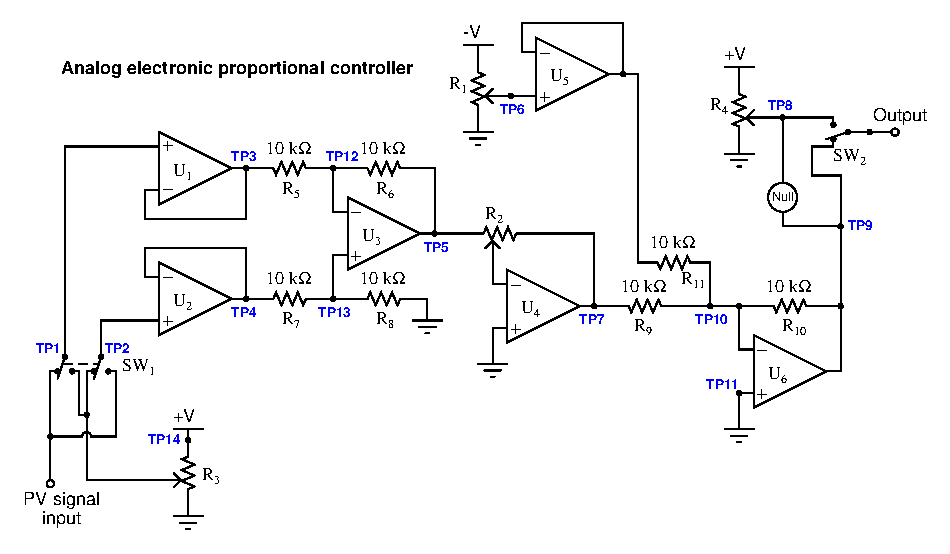
\includegraphics[width=15.5cm]{i00897x01.eps}$$

\begin{itemize}
\item{} $V_{TP3}$ = \underbar{\hskip 50pt} volt
\vskip 10pt
\item{} Output = \underbar{\hskip 50pt} volt
\vskip 10pt
\item{} $V_{TP10}$ = \underbar{\hskip 50pt} volt
\vskip 10pt
\item{} $V_{TP5}$ = \underbar{\hskip 50pt} volt
\end{itemize}

\underbar{file i00897}
%(END_QUESTION)





%(BEGIN_ANSWER)

Hvert riktig svar er verdt 2.5 poeng:

\begin{itemize}
\item{} $V_{TP3}$ = {\bf 2.8} volt
\vskip 10pt
\item{} Output = {\bf 2.7} volt
\vskip 10pt
\item{} $V_{TP10}$ = {\bf 0} volt
\vskip 10pt
\item{} $V_{TP5}$ = {\bf -0.3} volt
\end{itemize}

%(END_ANSWER)





%(BEGIN_NOTES)

{\bf Denne oppgaven er ment kun for eksamen, ikke for arbeidsark!}.

%(END_NOTES)
